\chapter{不确定性分析和风险分析}
不确定性分析——通过对拟建项目具有较大影响的不确定性因素进行分析,计算基本变量的增减变化引起项目财务或经济效益指标的变化,找出最敏感的因素及其临界点,可以\textbf{预测项目可能承担的风险}。

通过不确定性分析可以找出\textbf{影响项目效益的敏感因素,确定敏感程度},但不知这种不确定性因素发生的可能性及影响程度,因而不能代替风险分析。

通过风险分析可以得到\textbf{不确定性因素发生的可能性以及给项目带来经济损失的程度}。

\section{盈亏平衡分析(Break-Even Analysis)}
\noindent\textbf{目的:}

找出各种不确定性因素变化的\textbf{临界值}(会影响方案取舍的数值),判断方案对不确定性因素变化的\textbf{风险承受能力},为决策提供依据。

\noindent{\textbf{种类-按是否考虑资金时间价值}}
\begin{figure}[H]
    \centering
    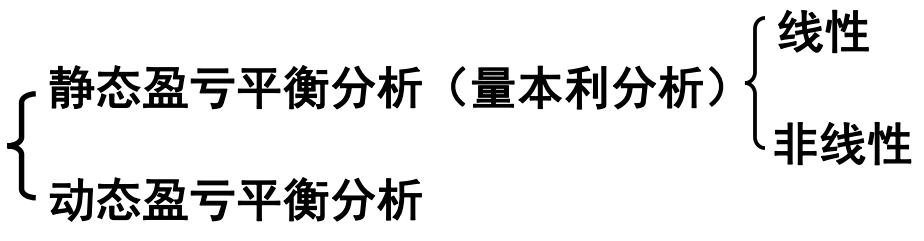
\includegraphics[width=0.7\textwidth]{image/盈亏平衡分析-种类.png}
    \label{fig:19}
\end{figure}

\subsection{线性静态盈亏平衡分析}
\subsubsection{含义}
分析\textbf{产量、成本与利润}之间的关系,找出投资方案\textbf{盈利或亏损}在产量、产品价格、单位产品成本等方面的\textbf{界限值},以判断在各种不确定因素作用下方案的风险状况(承受能力)。

\subsubsection{成本分类-按成本与产量的关系}
固定成本(Fixed costs, FC):在一定的产量范围内,\textbf{不随产量变动而变动}的成本。如设备折旧费等。

变动成本(Variable costs, VC):随产量的变动而变动的成本,如原材料等。通常假设变动成本与产量成正比关系,即:\textbf{变动成本 = 单位变动成本×产量}

\subsubsection{收入、成本、利润之间的关系}
1、年销售收入=价格×年产量=P×Q(假设销售价格不变,生产量=销售量)

2、年总成本=固定成本+变动成本=固定成本+单位变动成本×年产量=FC+v×Q 

3、年利润=年销售收入-年总成本= P×Q-(FC+v×Q)\\


\subsubsection{举例}
某投资项目需固定资产投资60万元,流动资金投资8万元,均在现在投入,项目当年建成投产,寿命期8年。项目的设计生产能力为生产产品10万件,预计价格7.5元/件,单位变动成本为4元/件,固定成本(未包括折旧)为每年10万元。假设项目固定资产投资全部形成固定资产原值,采用直线法折旧,折旧年限为8年,残值为0。

\textbf{原始资料:}
目前预计各参数数值:
\begin{itemize}
    \item 年设计生产能力10万件
    \item 产品价格7.5元/件
    \item 产品单位变动成本4.0元/件
    \item 固定成本:年折旧=60/8=7.5万元;年固定成本=10+7.5=17.5万元
\end{itemize}

根据上述资料,分别进行产量、价格、单位变动成本盈亏平衡点分析。\\
\textbf{1、产量盈亏平衡点分析}

在一定的价格、固定成本和单位变动成本下,使年利润为零的年产量。
$$P \times Q - (FC + v \times Q) = 0$$
$$Q^*=\frac{FC}{P-v}$$

若FC占总成本比例越大,则$Q^*$越高,即项目的风险性增大。

在本例中,$Q^*=\frac{17.5}{7.5-4.0}=5$(万件)

结论:
通过计算产量盈亏平衡点,可以对方案发生亏损的可能性作出大致判断。即项目的年产量只要达到或超过5万件,项目就不会亏损。

\begin{figure}[H]
    \centering
    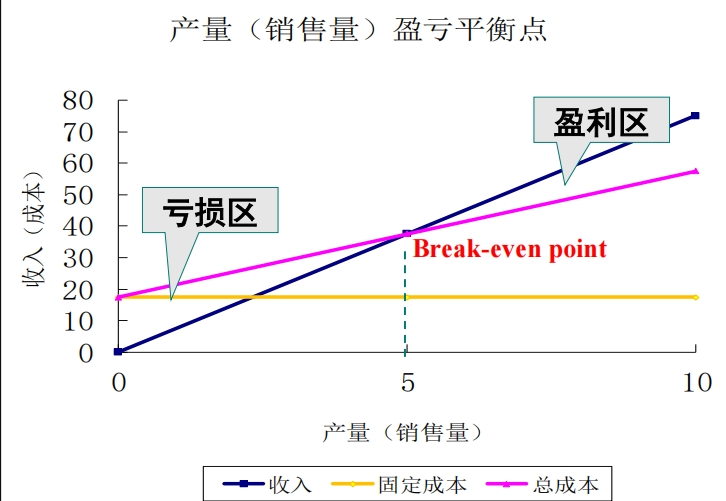
\includegraphics[width=0.75\textwidth]{image/盈亏平衡分析.png}
    \label{fig:20}
\end{figure}

盈亏平衡生产能力利用率:反映盈亏平衡产量占设计生产能力$Q_C$的比率。

$$E^*=\frac{Q^*}{Q_C} \times 100\% =\frac{5}{10} \times 100\% = 50\%$$

说明该项目年产量只要达到或超过设计生产能力的50\%,项目就不会亏损。\\\textbf{2、价格盈亏平衡点分析}

在固定成本和单位变动成本不变、按设计生产能力生产的情况下,使年利润为零的产品价格。

$P \times Q - (FC+v \times Q)=0$

$P* = \frac{FC}{Q_C}+v$

若FC占总成本比例越大,则$P^*$越高,即项目的风险性越大。

在本例中,$P^* = \frac{17.5}{10}+ 4.0 = 5.75$(元/件)

说明该项目产品的价格只要不低于5.75元/件,项目就不会亏损。

\begin{figure}[H]
    \centering
    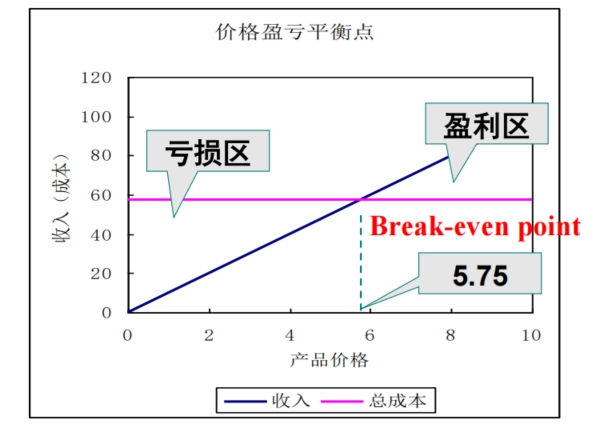
\includegraphics[width=0.75\textwidth]{image/静态盈亏平衡分析.png}
    \label{fig:21}
\end{figure}

\noindent \textbf{3. 单位变动成本盈亏平衡分析}

在产品价格和固定成本不变、按设计生产能力生产的情况下,使年利润为零的单位变动成本。

$P×Q-(FC+v×Q)=0$

$v^*=P-\frac{FC}{Q_C}$

若FC占总成本比例越大,则$V^*$越低,即项目的风险性越大。

在本例中,$v^*=7.5-\frac{17.5}{10}=5.75$(元/件)

说明该项目产品的单位变动成本只要不高于5.75元/件,项目就不会亏损。

\begin{figure}[H]
    \centering
    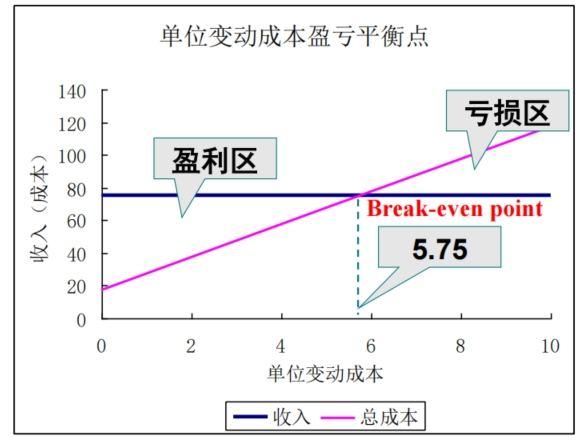
\includegraphics[width=0.75\textwidth]{image/单位变动成本盈亏平衡点.png}
    \label{fig:22}
\end{figure}

\subsubsection{成本结构与经营风险(自学范围,应该不考)}
理解结论的推导过程由销量及成本变动引起的经营风险的大小与项目固定成本占总成本费用的比例有关即可。

\subsubsection{静态盈亏平衡分析总结}
盈亏平衡分析的目的是找出临界值,即盈亏平衡点(BEP),判断投资方案对不确定因素变化的承受能力,为决策提供依据。

价格、产量盈亏平衡点越低,单位变动成本盈亏平衡点越高,说明项目盈利的可能性越大,亏损的可能性越小,因而项目有较大的抗经营风险能力。

\subsubsection{静态盈亏平衡分析的缺点}
(1)注重的是项目生产期的年利润,而没有考察项目的价值(没有考虑资金时间价值)。

(2)不适于分析生产期各年产量(销售量)不稳定的项目。

(3)分析较为笼统,只知道因素变化多大会使项目由盈利转为亏损。但因素的变化到底会使评价指标变化程度有多大还不知道。

\subsection{非线性静态盈亏平衡分析}
成本TC在实际中并不随产量呈直线变化,销售收入TR也受市场和用户的影响不呈线性变化。常见的是二次曲线型盈亏平衡分析。

\begin{figure}[H]
    \centering
    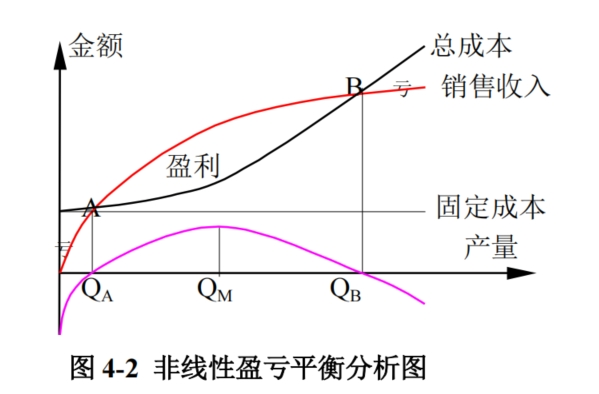
\includegraphics[width=0.7\textwidth]{image/非线性盈亏平衡分析图.png}
    \caption{非线性盈亏平衡分析图}
    \label{fig:23}
\end{figure}

设销售收入函数为f(x),成本函数为g(x),利润函数为 m(x)=f(x)-g(x)

解方程f(x)=g(x)得到的解为盈亏平衡时的产量。

令:

$$\frac{dm(x)}{d(x)}=\frac{d[f(x]-g(x)}{dx}=0$$

可得到最大利润所对应的产量$Q_M$及最大利润值。

例:某公司投资生产一种新产品,预计该产品的年销售收入$TR=3100Q-0.6Q^2$,年总成本$TC=3187500+600Q-0.2Q^2$。试求其盈亏平衡点的产量及利润最大化的产量。

当达到盈亏平衡点时,TR=TC,即:
$$3100Q-0.6Q^2=3187500+600Q-0.2Q^2$$
$$0.4Q^2-2500Q+3187500=0$$

\section{动态盈亏平衡分析}
\subsection{含义}
以项目的净现值为零,分析产量、价格、单位变动成本的变动临界点,从而判断项目在各种不确定因素作用下的风险状况。

即NPV=0时,分析

(1)在产品价格、单位变动成本、固定成本不变时,求年产量$Q^*$。

(2)在年产量为设计产量、单位变动成本和固定成本不变时,求产品价格$P^*$。

(3)在年产量为设计年产量、产品价格和固定成本不变时,求单位变动成本$v^*$。

\textbf{举例(原例续):}
某投资项目需固定资产投资60万元,流动资金投资8万元,均在现在投入,项目当年建成投产,寿命期为8年。项目的设计生产能力为生产某种产品10万件,预计产品价格为7.5元/件,单位变动成本为4元/件,固定成本(未包括折旧)为每年10万元。假设项目固定资产投资全部形成固定资产原值,采用直线法折旧,折旧年限为8年,残值为0。

\textbf{公司所得税税率为40\%,基准折现率为15\%。}(新增内容)

\textbf{解:}

初始现金流:-68万元

\noindent \textbf{营业现金流:}\\
收入:P×Q\\
变动成本:v×Q\\
固定成本:17.5万元\\
年利润:$(P-v)×Q-17.5$\\
年税后利润:$0.60 (P-v)×Q - 10.5$(年利润×0.6)\\
年营业现金流:$0.60 (P-v)×Q-3$(年利润+年折旧)

\begin{figure}[H]
    \centering
    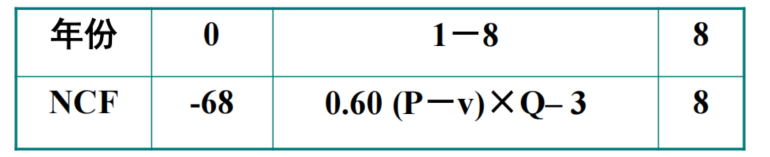
\includegraphics[width=0.75\linewidth]{image/表1.png}
\end{figure}

\noindent 令NPV = 0,
$$-68 +[0.60 \times (P − v) \times Q − 3](P/ A,15\%,8) + 8(P/ F,15\%,8) = 0$$
$$− 28.87 + (P −v) \times Q = 0$$
求得产量盈亏平衡点:8.24万件;价格盈亏平衡点:6.89元/件;单位变动成本盈亏平衡点:4.61元/件;终结现金流:8万元。

\noindent \textbf{结论:}

当产品价格为7.5元/件,单位变动成本为4.0元/件,年固定成本为17.5万元时,项目的年产量只要达到或超过8.24万件/年,或生产能力利用率达到或超过82.4\%,项目就有经济价值。

当项目按设计生产能力10万件/年进行生产,单位变动成本为4.0元/件,年固定成本为17.5万元时,产品价格只要达到或超过6.89元/件,项目就有经济价值。

当项目按设计生产能力10万件/年进行生产,产品价格为7.5元/件,年固定成本为17.5万元时,单位变动成本只要不超过4.61元/件,项目就有经济价值。

\noindent \textbf{例:}(单选)关于盈亏平衡分析,说法错误的是\\
A.盈亏平衡价格越高,项目的风险承受能力越高。\\
B.盈亏平衡产量越高,项目的风险承受能力越低。\\
C.盈亏平衡生产能力利用率越低,项目的风险承受能力越高。\\
D.固定投资占总成本比例越大,项目的风险性越大。\\
\textbf{答案:}A。

\section{敏感性分析}
\subsection{含义}
通过测定一个或多个不确定因素的\textbf{变化}所导致的决策评价指标的\textbf{变化幅度},了解各种因素的变化对实现预期目标的\textbf{影响程度},从而对外部条件发生不利变化时投资方案的\textbf{承受能力}作出判断。

\subsection{作用}
研究相关因素的变动引起经济效果评价指标的变动幅度;

找出敏感性因素,预测其可能产生的不确定性对方案的影响,以便采取控制措施;

敏感性分析结论有助于方案选优。

\subsection{种类:按所分析不确定性因素的个数}

\subsubsection{单因素敏感性分析(重点)}
假定其他因素不变,分析某一不确定因素的变动对方案经济效果产生的影响。\\
\textbf{(一)分析步骤}

1、选择需要分析的不确定因素,并设定这些因素的变动范围;

2、确定分析指标;

3、进行敏感性计算,建立敏感性分析表和分析图;

4、确定敏感因素,即其数值变动能显著影响方案经济效果的因素。

\noindent \textbf{(二)举例(续):}

假设上述投资项目中固定资产投资、产量、产品价格、单位变动成本等是不确定因素,这些因素都有可能偏离预计值-20\%到+20\%。分析哪些因素是敏感因素。

\begin{figure}[H]
    \centering
    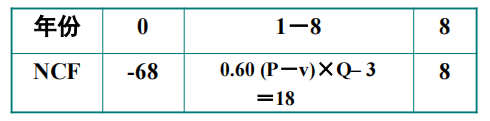
\includegraphics[width=0.85\linewidth]{image/单因素-例题.png}
\end{figure}

\textbf{1、基础方案}

固定资产投资60万元,流动资金投资8万元,年产量10万件,产品价格7.5元/件,单位变动成本4.0元/件,固定成本(不包含折旧)10万元/年,折旧7.5万元/年
$NPV=15.39$万元
$IRR=21.39\%$

\textbf{2、选定不确定因素,设定可能的变动范围}

固定资产投资、产量、产品价格、单位变动成本

变动范围为-20\%到+20\%

\textbf{3、确定分析的指标}:净现值NPV。

\textbf{4、敏感性计算及结果}

\begin{figure}[H]
    \centering
    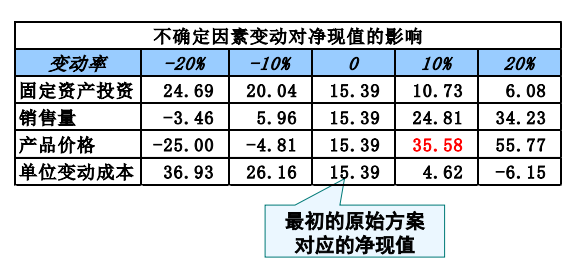
\includegraphics[width=1\linewidth]{image/不确定因素变动对净现值的影响.png}
\end{figure}

\begin{figure}[H]
    \centering
    \caption{产品价格变动10\%时,净现值的计算举例:}
    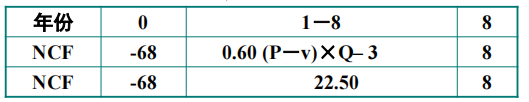
\includegraphics[width=0.85\linewidth]{image/净现值的计算举例.png}
\end{figure}

1-8年每年净现金流$= 0.60 (P-v) \times Q - 3 = 0.60 \times (7.5 \times 1.1 - 4) \times 10 - 3 = 22.50$

净现值$=-68+22.5 \times (P/A,15\%,8)+8 \times (P/F,15\%,8) = 35.58$

(目前预计价格7.5,产量10,单位变动成本4)

\begin{figure}[H]
    \centering
    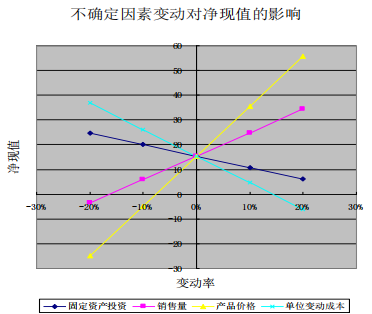
\includegraphics[width=0.8\linewidth]{image/敏感性计算及结果图示.png}
    \caption{敏感性计算及结果图示}
\end{figure}

\textbf{这个图很重要,斜率绝对值最大的对净现值影响最大。}

\textbf{5、判定敏感因素}

\noindent \textbf{相对测定法}

比较在同一变动幅度下各因素的变动,对经济效果指标产生的影响,据此判断方案经济效果对各因素变动的敏感程度。

\begin{figure}[H]
    \centering
    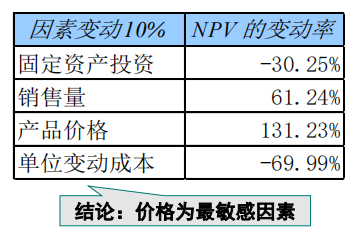
\includegraphics[width=0.75\linewidth]{image/相对测定法.png}
\end{figure}

\textbf{敏感度系数=项目评价指标变化率/不确定性因素变化率}

\noindent \textbf{绝对测定法}

测定使经济效果指标达到临界值时各因素的变动幅度,变动幅度越小,则方案的经济效果对该因素越敏感。

\begin{figure}[H]
    \centering
    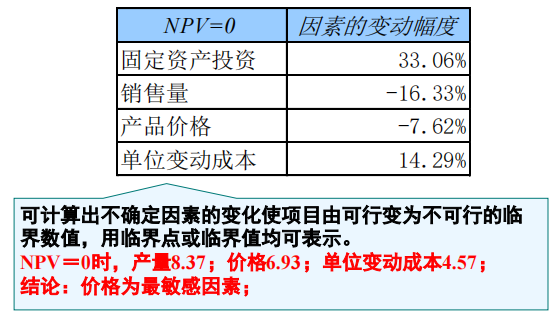
\includegraphics[width=0.75\linewidth]{image/绝对测定法.png}
\end{figure}

\textbf{例1:}(多选)关于敏感性分析,说法错误的是
A.单因素敏感性分析图中,影响因素直线斜率越小,该因素越敏感
B.比较在同一变动幅度下各因素的变动,对经济效果指标产生的影响越大,该因素越敏感
C.测定使经济效果指标达到临界值时各因素的变动幅度,变动幅度越小,该因素越敏感
D.敏感性分析没有考虑各种不确定性因素在未来发生变动的概率

\textbf{例2:}单因素敏感性分析中,甲、乙、丙、丁四因素分别发生5\%、10\%、10\%、15\%的变动,经济效果评价指标均发生20\%的变动,最敏感的因素是?

\textbf{答案:}甲。



\subsubsection{多因素敏感性分析(不重要)}
分析多个因素同时变动对方案经济效果的影响。

\noindent \textbf{1.引入-单因素敏感性分析的局限性}

单因素敏感性分析,计算某一因素变动对经济效果指标的影响时,假定其他因素均不变。

但实际上,一个因素的变动往往也伴随着其他因素的变动。

如:产品价格上涨时,产品需求量可能下降。

解决方法:引入多因素敏感性分析。

\noindent \textbf{2.特点:}

多因素敏感性分析需要考虑可能发生的各种因素不同变动幅度的多种组合,计算起来相对复杂的多。

如果需要分析的不确定性因素不超过三个,可以用解析法和作图法相结合的方法进行。

\subsection{敏感性分析评价}
敏感性分析在一定程度上,就各种不确定性因素的变动对经济效果的影响作了定量描述。有助于帮助确定在决策过程中,需要重点研究和控制的因素。

但敏感性分析没有考虑各种不确定性因素在未来发生变动的概率,可能会影响分析结论的正确性。

如通过敏感性分析找出的某一敏感因素,在未来发生不利变动的概率很小,因而实际上所带来的风险并不大。

解决办法:进行概率分析。

\section{概率分析}
看看得了,我觉得不考。

\section{风险决策(理解决策原则)}
\subsection{引入}
概率分析可以给出方案经济效果指标的期望值和标准差,以及指标的实际值发生在某一区间的概率。但是概率分析没有给出风险条件下,方案取舍的原
则和多方案比选的方法。

\subsection{风险决策条件}
1、存在着两个或两个以上可供选择的方案;

2、存在两种或两种以上的随机自然状态;

3、已知各种自然状态出现的概率;

4、已知各种自然状态下,各方案经济效果指标的估值;

5、存在着决策人希望达到的目标(收益最大/损失最小)

\subsection{举例}
某企业拟开发一种新产品取代将要滞销的老产品。技术部门提出了三种方案,新产品投入市场后可能出现四种前景。已经估计了每种前景出现的概率,各方案在每种前景下可能的净现值,决策者要解决的问题是应该选择哪个方案。

\begin{figure}[H]
    \centering
    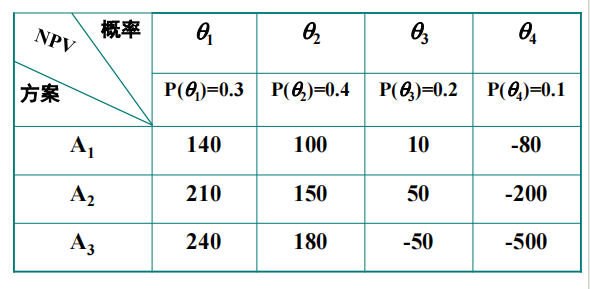
\includegraphics[width=0.75\linewidth]{image/风险决策-选哪个方案.png}
\end{figure}

\subsection{风险决策原则(可能考选择或简答)}
优势原则、期望值原则、最小方差原则、最大可能原则、满意原则。

\subsubsection{(1)优势原则}
在互斥方案A、B中,如果不论在什么状态下A总是优于B,则可以认定A相对于B是优势方案,从而剔除B。

应用优势原则一般不能决定最佳方案,但能够减少备选方案的数目。

在采用其他决策原则进行方案比选之前,应首先运用优势原则剔除劣势方案。

\subsubsection{(2)期望值原则}
选择净现值的期望值最大的方案,或费用现值的期望值最小的方案。

在上例中,按照期望值原则应选择A2。

$E(NPV)1=76$万元

$E(NPV)2=113$万元

$E(NPV)3=84$万元

\subsubsection{(3)方差最小原则}
选经济效果指标的方差最小的方案。

在上例中,按照方差最小原则应选择A1。

$D(NPV)1=4764$万元

$D(NPV)2=13961$万元

$D(NPV)3=48684$万元

与期望值原则得出的结论不同。

\subsubsection{(4)最大可能原则}
如果一种状态发生的概率显著大于其他状态,那么就把这种状态视作肯定状态,根据这种状态下各方案的经济效果指标来进行决策。

按照最大可能原则决策实际上将风险决策问题转化为确定性决策问题。

\noindent \textbf{注意:适用前提:}

1、一种状态发生的概率显著大于其他状态;

2、各方案在不同状态下的损益值的差别不很悬殊;

\textbf{按最大可能原则分析上例:}

状态$\theta 2$发生的概率最大,如果按照最大可能原则决策,应选择$\theta 2$下净现值最大的A3方案。

\begin{figure}[H]
    \centering
    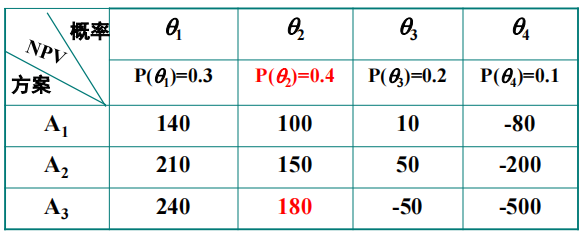
\includegraphics[width=0.75\linewidth]{image/最大可能原则分析.png}
\end{figure}

但从本例的适用前提来看,

$\theta 2$发生的概率P($\theta 2$)=0.4,与其他状态发生的
概率差别不大;A3方案在不同状态下净现值相差较大。

即最大可能原则在本例中不太适用。

\noindent\textbf{(5)满意原则}
定出一个足够满意的目标值,将各备选方案在不同状态下的经济效果指标与此目标值进行比较,选择经济效果指标优于或等于目标值的概率最大的方案。

上例中如果满意目标是净现值不小于30万元,则应该选择A2。

P(NPV $\geq$ 30)1=P($\theta 1$)+ P($\theta2$)=0.7

P(NPV $\geq$ 30)2= P($\theta 1$)+ P($\theta2$) + P($\theta3$) =0.9

P(NPV $\geq$ 30)3=P($\theta 1$)+ P($\theta2$)=0.7

\section{决策方法}
决策原则:期望值原则。

矩阵法(不重要)、\textbf{决策树法}

\subsection{含义}
一种由不同节点和分枝组成的树型决策网络,它描述了风险决策的所有要素,包括备选方案、状态、状态发生的概率、备选方案在各种状态下的损益值,据此可以判断出应该选择哪个方案。决策树中常用方块表示决策节点,用圆圈表示状态节点。

\textbf{例1:}
某石油公司正在决策是否在某一地区钻井。

\textbf{备选方案:}钻井、不钻井

\textbf{可能的状态:}成功、失败(干井)

\textbf{概率:}成功的概率为0.60,失败的概率为0.40。

\textbf{净现值:}

如果成功,净现值等于600万美元;

如果失败,净现值等于-200万美元。

\begin{figure}[H]
    \centering
    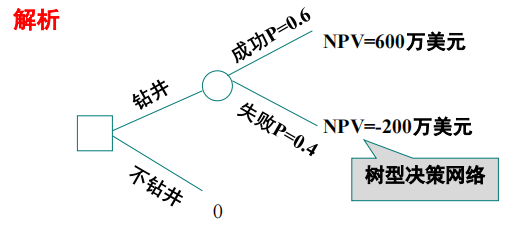
\includegraphics[width=\linewidth]{image/决策树.png}
\end{figure}

某勘探项目面临如下决策:是否购买区块?购买后,是直接钻井,还是先进行地震勘探?如果第一口井是干井,是否钻第二口井?

\noindent \textbf{基础资料}
\noindent \textbf{(1)成本收益数据}
大发现的价值=\$40

小发现的价值=\$15

区块购买成本=\$3

钻井成本=\$1

地震勘探成本=\$2

\noindent \textbf{(2)概率数据}
\textbf{直接钻井情况下(若第一口井为干井,才考虑是否钻第二口井。)}

大发现:第一口井概率5\%,第二口井概率7.5\%;

小发现:第一口井概率5\%,第二口井概率7.5\%;

干井:第一口井概率90\%,第二口井概率为85\%。

\textbf{先进行地震勘探后再钻井情况下地震勘探后发现有潜在油藏的概率为50\%,若第一口井为干井,才考虑是否钻第二口井。}

大发现:第一口井概率15\%,第二口井概率20\%;

小发现:第一口井概率15\%,第二口井概率20\%;

干井:第一口井概率70\%,第二口井概率为60\%。

\begin{figure}[H]
    \centering
    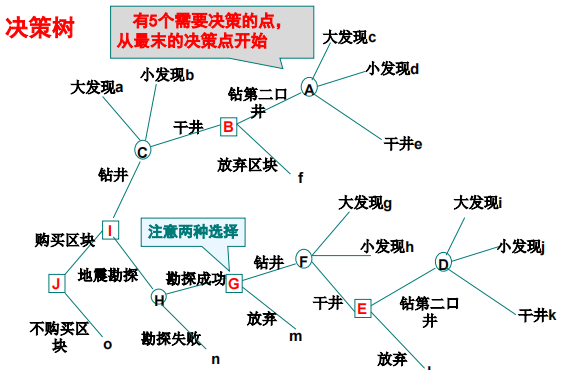
\includegraphics[width=1\linewidth]{image/决策树1-例1.png}
\end{figure}

\begin{figure}[H]
    \centering
    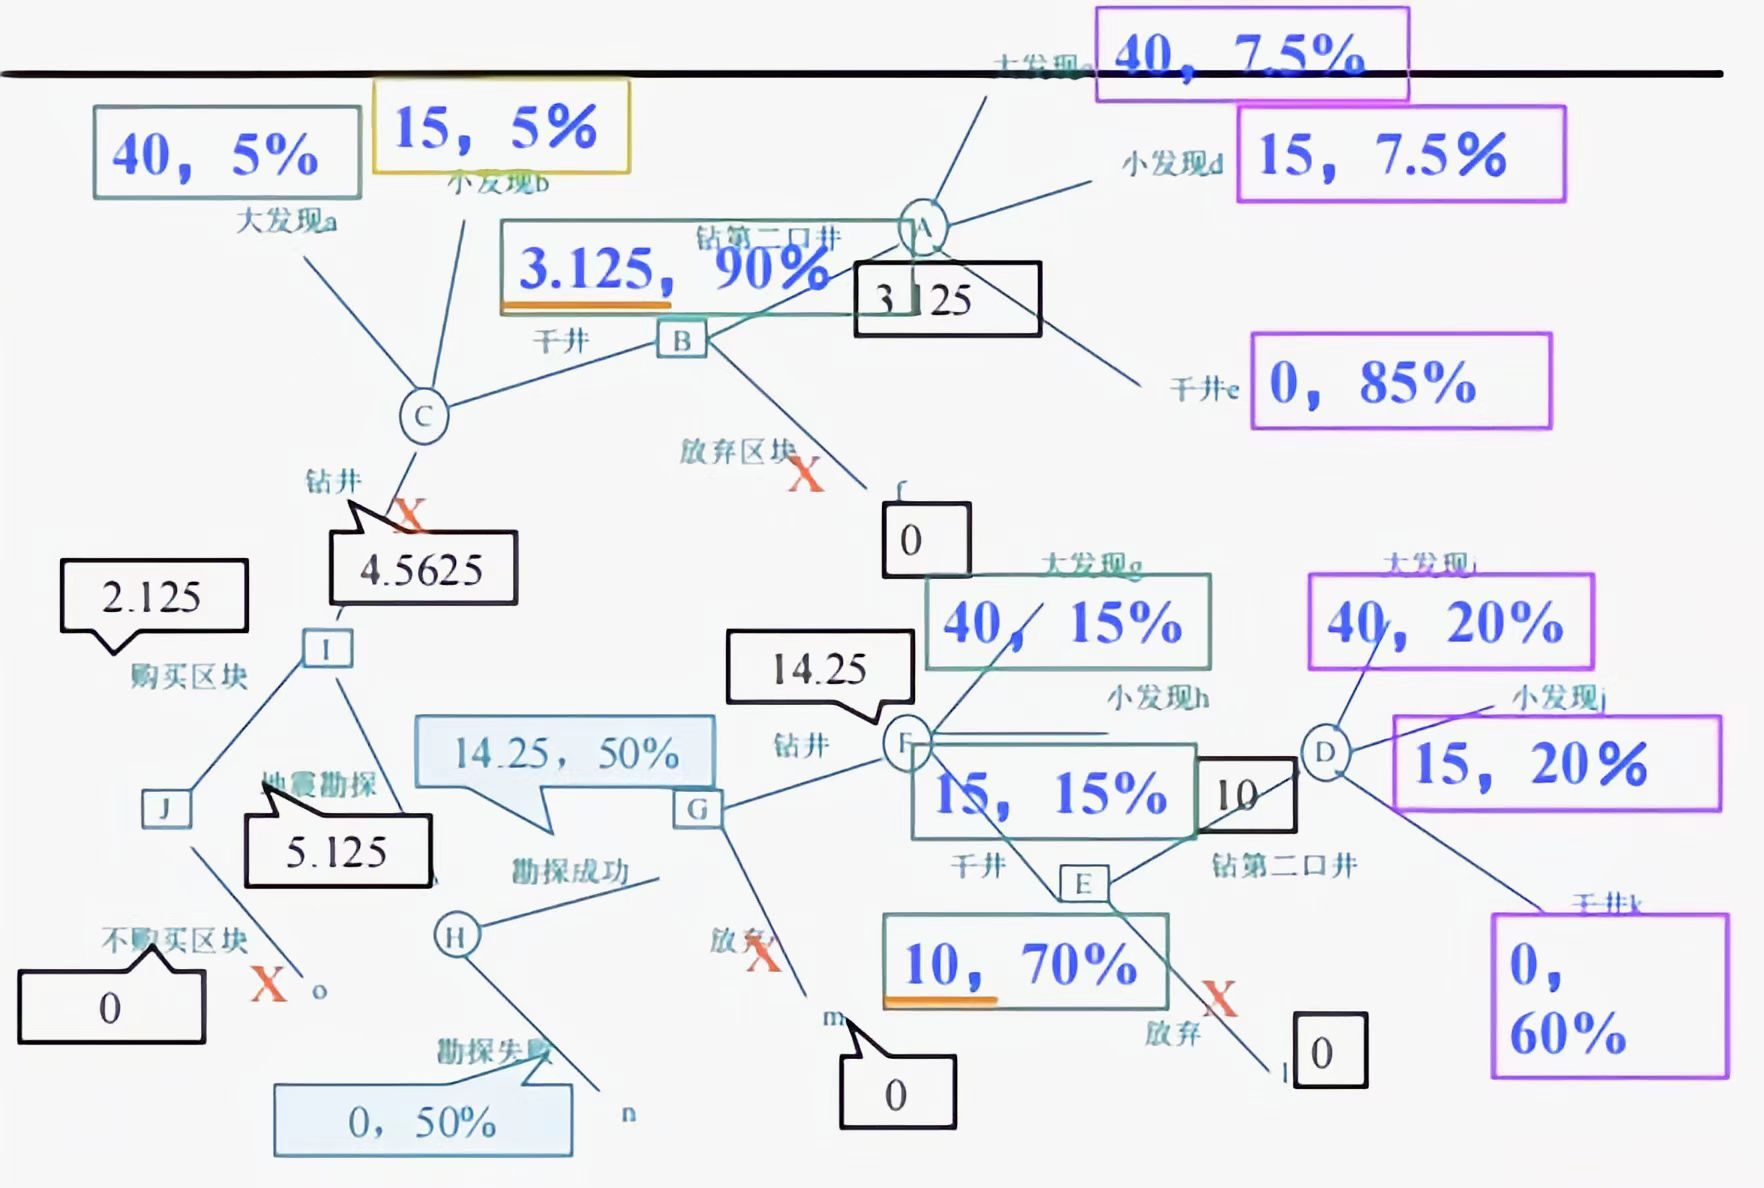
\includegraphics[width=1\linewidth]{image/决策树2-例1.jpg}
\end{figure}

\noindent \textbf{解析:}

利用决策树进行多阶段风险决策,要从最末一级决策点开始。

\textbf{(1)决策点B}

状态点A的期望净现值:

$ENPV_A=-\$1+(\$40×0.075+\$15×0.075+\$0×0.85)=\$3.125$

与放弃(净现值为零)相比,应该决策钻第二口井。

\textbf{(2)决策点E}

状态点D的期望净现值:

$ENPV_D=-\$1+(\$40×0.20+\$15×0.20+\$0×0.60)=\$10$

与放弃(净现值为零)相比,应该决策钻第二口井。

\textbf{(3)决策点G}

状态点F的期望净现值:

$ENPV_F=-\$1+(\$40×0.15+\$15×0.15+\$10×0.70)=\$14.25$

(注意:用状态D的期望净现值代替E决策点)

与放弃(净现值为零)相比,应该决策钻第一口井。

\textbf{(4)决策点I}

状态点C的期望净现值:

$ENPV_C=-\$1+(\$40×0.05+\$15×0.05+\$3.125×0.90)=\$4.5625$

状态点H的期望净现值:

$ENPV_H=-\$2+(\$14.25×0.50+\$0×0.50)
=\$5.125$

状态点C与状态点H相比,应该选择地震勘探。

\textbf{(5)决策点J}

购买区块的期望净现值$=-\$3+\$5.125=\$2.125$

与不购买(净现值为零)相比,应该选择购买。

\textbf{(6)决策结论}

通过决策树分析,决策结果如下:

购买区块;先进行地震勘探;如果勘探成功,钻第一口井;如果第一口井是干井,继续钻第二口井。

\begin{figure}[H]
    \centering
    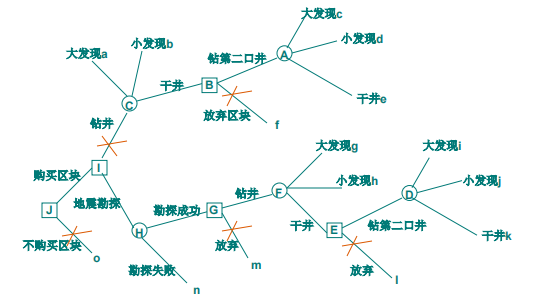
\includegraphics[width=1\linewidth]{image/决策结果.png}
\end{figure}